\documentclass[aspectratio=169]{beamer}

\usetheme{UiO}

\usepackage{emoji}

\title{En introduksjon til kunstig intelligens}
\subtitle{Og dets rolle i medisinsk forskning}
\author{Esten H. Leonardsen}
\date{\today}


\begin{document}
	\begin{frame}
	 	\titlepage
	\end{frame}

    \begin{frame}{Hva er kunstig intelligens?}
        \begin{tikzpicture}
            \node[draw=black] at (-7, -3.25) {};
            \node[draw=black] at (7, 3.25) {};

            \visible<1>{
                \node[anchor=west, inner sep=0pt, draw=black, label=below:\tiny{ChatGPT}] at (-7, 0) {
                    
\includegraphics[width=4.1cm]{data/chatgpt.png}
                };
                \node[inner sep=0pt, draw=black, label=below:\tiny{Spot}] at (-0.5, 1.5) {
                    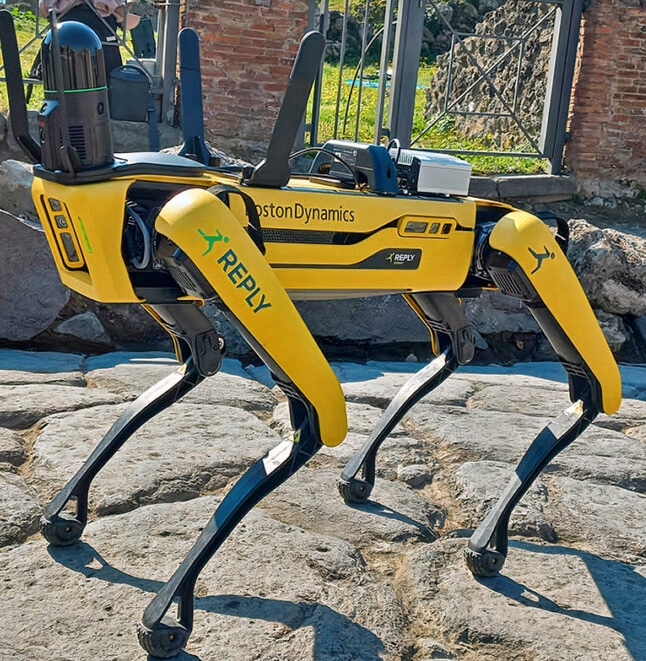
\includegraphics[width=3cm]{data/spot.jpg}
                };
                \node[inner sep=0pt, draw=black, label=below:\tiny{Sophia}] at (2.7, 1.5) {
                    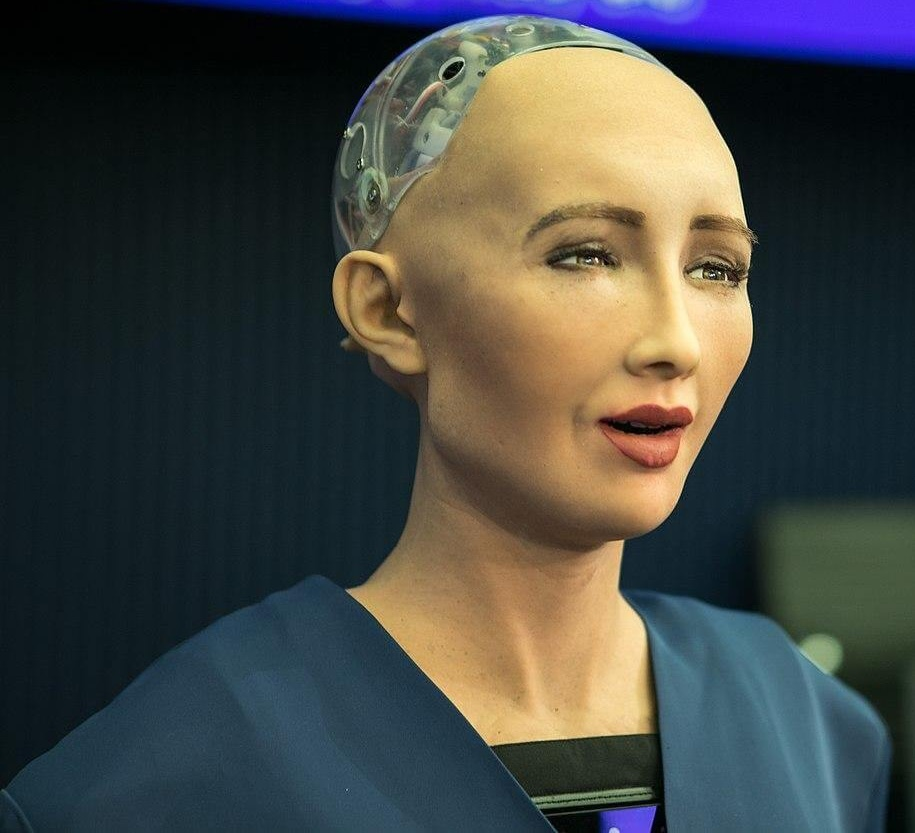
\includegraphics[width=3cm]{data/sophia.jpg}
                };
                \node[inner sep=0pt, draw=black, label=below:\tiny{AlphaFold}] at (1, -1.5) {
                    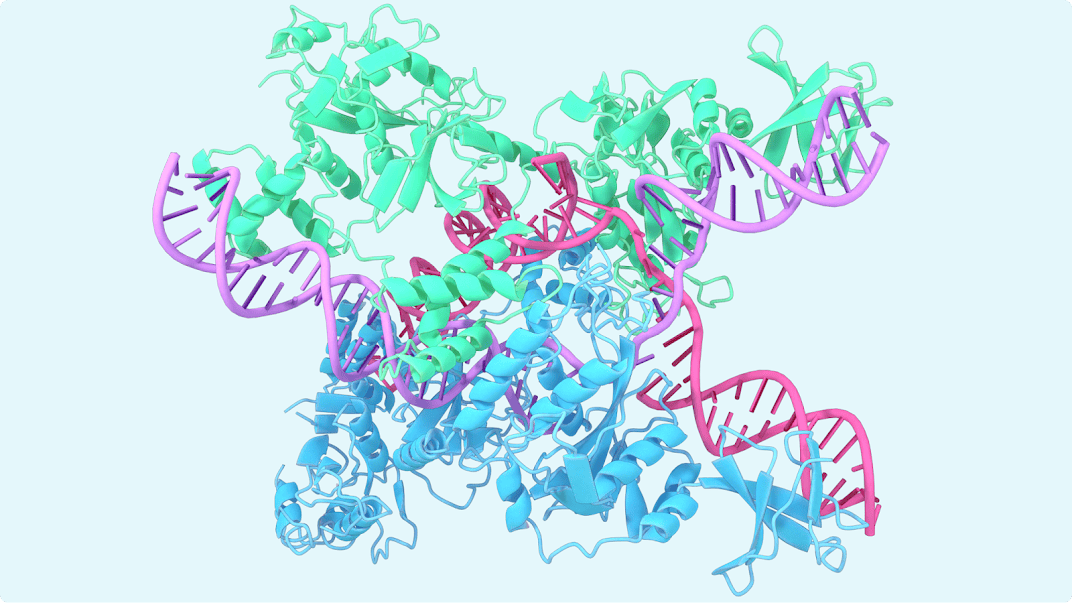
\includegraphics[width=4cm]{data/alphafold.png}
                };
            }

            \visible<2-4,9>{
                \node[circle, fill=blue!60, minimum size=6cm, anchor=north] (ai) at (-4, 3.25) {};
                \node[white, anchor=north, align=center, font=\small\bfseries\linespread{0.9}\selectfont] at ($ (ai.north) - (0, 0.1) $) {Kunstig\\intelligens};

                \visible<2>{
                    \node[align=flush left, anchor=north west, text width=7.2cm, font=\small\linespread{0.95}\selectfont] (def1) at (-0.5, 3.25) {
                        \textbf{Kunstig intelligens}\\
                        Teknologi som løser oppgaver som krever en eller annen form for intelligens
                    };
                }
                \visible<3->{
                    \node[align=flush left, anchor=north west, text width=7.2cm, font=\small\linespread{0.95}\selectfont] (def1) at (-0.5, 3.25) {
                        \textbf{Kunstig intelligens}\\
                        Et fagfelt som produserer teknologi som løser oppgaver som krever en eller annen form for intelligens
                    };
                }

                \visible<4->{
                    \node[align=center, font=\small\linespread{0.9}\selectfont, text=white] at ($ (ai.north) + (1.3, -1.5) $) {Regelstyrte\\systemer};
                }

                \visible<9->{
                    \node[circle, fill=purple!60, anchor=south, minimum size=4.1cm] (ml) at ($ (ai.south) + (0, 0.05) $) {};
                    \node[white, anchor=north, align=center, font=\small\bfseries\linespread{0.9}\selectfont] at ($ (ml.north) - (0, 0.3) $) {Maskinlæring};
                }
                \visible<12->{
                    \node[align=flush left, anchor=north west, text width=7.2cm, font=\small\linespread{0.95}\selectfont] (def2) at (def1.south west) {
                        \textbf{Maskinlæring}\\
                        Teknologi som lærer seg å løse problemer ved å finne nyttige mønstre i treningsdata
                    };
                }
            }
            \visible<5-8>{
                \def\systemfont{\footnotesize}

                \node[draw=black, fill=gray!90, minimum width=6cm, minimum height=2cm, rounded corners=0.1cm, text=white, text depth=2.35cm, font=\systemfont] (system) at (0, 1) {Ekspertsystem};

                \visible<6->{
                    \node[draw=black, label=below:\systemfont{Prediksjon}, anchor=west] (output) at ($ (system.south east) + (1, 0.9825) $) {
                        \systemfont{Influensa}
                    };

                    \node[] (notepad) at ($ (system.south west) + (-1, 0.9825) $) {\Large{\emoji{spiral-notepad}}};
                    \node[anchor=east, inner sep=-2pt] at (notepad.west) {\Huge{\emoji{man-health-worker}}};

                    \draw[-stealth] (notepad.east) -- ($ (system.south west) + (0, 0.9825) $);
                    \draw[-stealth] ($ (system.south east) + (0, 0.9825) $) -- (output);
                }

                \visible<7->{
                    \node[fill=gray!80, minimum width=4cm, minimum height=2.3cm, rounded corners=0.1cm, text=white, text depth=1.8cm, draw=black, font=\systemfont, anchor=south] (rule) at ($ (system.south) + (0, 0.05) $) {Regelmotor};
                    \node[draw=black, fill=white, rounded corners=0.05cm, font=\systemfont, minimum width=1.7cm, minimum height=0.55cm, anchor=south] (symptom1) at ($ (rule.south) + (0, 1.25) $) {Feber};
                    \node[draw=black, fill=white, rounded corners=0.05cm, font=\systemfont, minimum width=1.7cm, minimum height=0.55cm, anchor=south] (symptom2) at ($ (rule.south) + (0, 0.65) $) {Hoster};
                    \node[draw=black, fill=white, rounded corners=0.05cm, font=\systemfont, minimum width=1.7cm, minimum height=0.55cm, anchor=south] (symptom3) at ($ (rule.south) + (0, 0.05) $) {Sår hals};

                    \draw[-stealth] ($ (system.south west) + (0, 0.9825) $) -- ($ (rule.south west) + (0, 0.9325) $);
                    \draw[-stealth] ($ (rule.south west) + (0, 0.9325) $) -- (symptom1.west);
                    \draw[-stealth] ($ (rule.south west) + (0, 0.9325) $) -- (symptom2.west);
                    \draw[-stealth] ($ (rule.south west) + (0, 0.9325) $) -- (symptom3.west);
                    \draw[-stealth] (symptom1.east) -- ($ (rule.south east) + (0, 0.9325) $);
                    \draw[-stealth] (symptom2.east) -- ($ (rule.south east) + (0, 0.9325) $);
                    \draw[-stealth] (symptom3.east) -- ($ (rule.south east) + (0, 0.9325) $);
                    \draw[-stealth] ($ (rule.south east) + (0, 0.9325) $) -- ($ (system.south east) + (0, 0.9825) $);
                }
                \visible<8>{
                    \node[] (expert) at ($ (system.south) - (0, 1.75) $) {
                        \Huge{\emoji{woman-scientist}}
                    };
                    \draw[-stealth, dashed] (expert) -- (rule.south);
                }
            }

            %     \node[circle, fill=red!60, anchor=south, minimum size=3cm] (dl) at ($ (ml.south) + (0, 0.06) $) {};
            %     \node[white, anchor=north, align=center, font=\small\bfseries\linespread{0.9}\selectfont] at ($ (dl.north) - (0, 0.1) $) {Dyp\\læring};
            % }
        \end{tikzpicture}
    \end{frame}
\end{document}
